%%
%% Author: mahmoud
%% 19/04/12
%%

\chapter{Folge und Reihen:}
\section{Folgen und Reihen}
\numberwithin{equation}{theorem}
\begin{definition}
    Ein folge ist eine Abbildung

    \[ f: \mathbb{N} \rightarrow \underbrace{\mathbf{M}}_{Menge} : \mathrm{n} \mapsto \underbrace{X_n}_{folgenglied} \]

\end{definition}
\begin{remark}

    \begin{align}	\mathbb{M} &= \mathbb{R} \quad reelewert Folge  \notag \\
    M&= \mathbb{C} \quad	 Komplexewetig folge  \notag \\
    \mathbb{M}&= \mathbb{R}^n \quad vertical folge \notag
    \end{align}




\end{remark}
\begin{description}

    \item[Bezeichnung]

    \quad $(X_n)$ \space \text{mit} \space $ \left( X_n =  \right) \frac{n}{n+1} $
    \\ \\ Aufzählung der folglieder: 0 , $\frac{1}{2}$ ,$\frac{2}{3}$ , $\frac{3}{4}$ , \dots
    \begin{remark}
        zuweten wird $\mathbb{N}$ durch $\mathbb{N}$ {0,1 \dots} erstellt.


    \end{remark}
    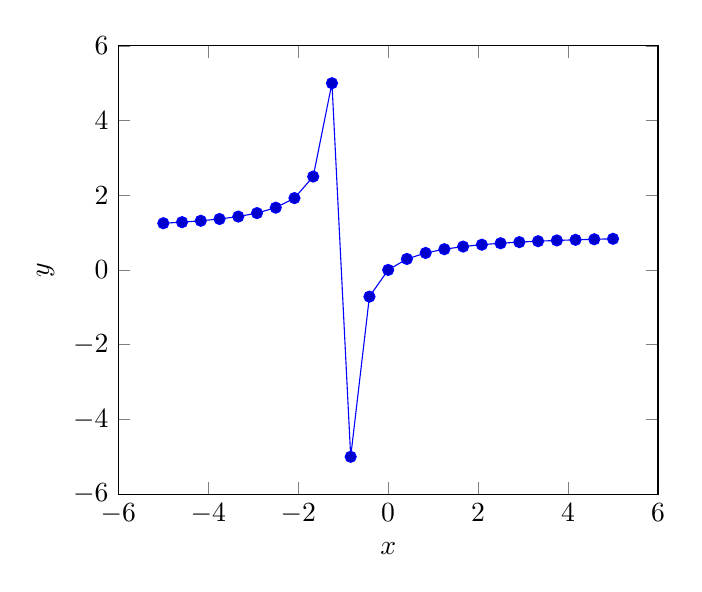
\begin{tikzpicture}
        \begin{axis}[
        xlabel= $x$,
        ylabel= {$y$}]
            \addplot { x/(x+1)};
        \end{axis}
    \end{tikzpicture}
\end{description}
\begin{example}
    \[\]
    \begin{enumerate}

        \item Konstante Folge $(X_n)$ mit \quad $X_n = a \in \mathbb{M },a \dots$ \\
        \[ X_n = a \in \mathbb{M} \]
        \item Harmonische Folge $(X_n)$  mit $X_n$ =  $\frac{1}{n+1}$ \quad$ n \geq 1$
        \item Geometrische folge $(X_n)$ mit $X_n = q^n \:. \: q \in \mathbb{R}, \dots $
        \item Fibonaccifolge $(X_n)$ mit
        \[ X_n =\frac{1}{\sqrt{5}} \Big(  \big( \frac{1+ \sqrt{5}}{2} \big)^n - \big( \frac{1- \sqrt{5}}{2}\big)^n   \Big)    \]

        \item Fibonacci folgen $(X_n)$
        \begin{align}
            X_0 &=0 \notag \\X_1 &= 1 \notag \\
            X_n+1 &= X_n+X_n-1 (n>0)  \notag
        \end{align}

        \item conway  folge
        \[ 1, 11 ,21 , 1211, 111217, 312211 \dots \]

        \item folge aller Primzahlen:- \[ 2, 3 ,5 ,7 ,11, 13 , \dots \]

    \end{enumerate}
\end{example}

\section{Rechnen mit Folgen }
\begin{align*}
    M  = \mathbb{R} \quad oder \quad M = \mathbb{C} \\
    (X_n)+(y_n) := (X_n+y_n)\\
    K(X_n):=(KX_n)\in \mathbb{R} \quad  oder \quad \in  \mathbb{C}
\end{align*}
\begin{remark}
    \[\]
    Die Folge bildet ein Vektorraum.
\end{remark}


\begin{definition}


    \begin{enumerate}

        \mbox{}\item Eine reellwertige Funktion ist in der Mathematik eine Funktion, deren Funktionswerte reelle Zahlen sind.

        \item Eine reellwertige heißt beschränkt wenn gilt

        \[	\exists r \in \mathbb{R}_+ , \forall r \in \mathbb{N}: \underbrace{|x|}_{\text{ Betrag einer reellen oder komplexer Zahl}} \leqq r   \]

    \end{enumerate}
\end{definition}

\begin{example}
    \[(X_n)\quad mit \quad X_n = (-1)^n \times \frac{1}{n} \]
    \[-1 ,\quad \frac{1}{2}, \quad \frac{-1}{3}, \quad \frac{1}{4} ,\quad \frac{-1}{5},\dots \]
\end{example}

\begin{remark}

    $(X_n)$ ist beschränkt mit $r = 1$ denn $|(-1)^n \frac{1}{n}|=|\frac{1}{n}| \leqq 1  $

\end{remark}

\begin{tikzpicture}
    \begin{axis}[
    ymin = -2,
    ymax = 2,
    xmin = -3,
    xmax = 3,
    axis x line=center,
    axis y line=center]
        \addplot[samples at={-3,...,3},only marks,mark size=1]{(-1)^x*(1/x)};
    \end{axis}
\end{tikzpicture}
\begin{example}
    \[  (X_n) mit X_n = (-1)^n \frac{1}{n}+1 \quad \text{bechränkt r = 3/2}\]

    \[-1/3 \quad \leq X_n \leq 3/2 \quad \forall n \in \mathbb{N} \]
    %
    \begin{tikzpicture}
        \begin{axis}[
        ymin = -2,
        ymax = 2,
        xmin = -4,
        xmax = 4,
        axis x line=center,
        axis y line=center]
            \addplot[samples at={-3,...,3},only marks,mark size=1][ domain=(-1/3):(3/2)] {((-1)^x)*(1/x)+1};
        \end{axis}
    \end{tikzpicture}
\end{example}
\vfil
\vfil
\begin{example}{Standard:}\\

{Die folge}
$ \bigg(\big(1 + \frac{1}{n} \big)^n \bigg)^\infty$
{ist beschränkt durch 3}\\

Zu Zeigen:

\[ -3 \leq X_n \leq 3 \quad \text{für alle} \quad n \in \mathbb{N} \]
\[ { (a+b)^n = \sum_{k=0}^{n} \binom{n}{k} a^k . b^{n .k} = \sum_{k=0}^{n} \binom{n}{k} a^{n.k} b^k }  \]
\[  \binom{n}{k} = \frac{n!}{k!(n-k!)} =  \frac{n(n-1) -(n-k-1))}{k!} \]
\[  \sum_{K=0}^{n} \frac{1}{k} = 1+ \frac{1}{2} + \frac{1}{2.3} + \frac{1}{2.3.4} + \dots \]
\end{example}


\section{geometrische Summen Formel (Tafelwerk)}
\begin{definition}

    Die Folge $(X_n)$ heißt monoton $\Big\{ wachsend fallend \Big\}$
    \[ wenn \quad gilt: \forall n \in \mathbb{N}:
    \left\{
    \begin{array}{ll}
        X_n  & \leq X_n +1 \\
        X_n  & \geq X_n+1
    \end{array}
    \right. \]
    \text{man spricht von Streng monotonie}
    $ wenn \leq durch > und \geq durch < \dots  $
\end{definition}
\begin{remark}
    \[ X_n \leq X_{n+1} \ \Leftrightarrow  X_n - X_{n+1} \geq 0 \quad \Leftrightarrow  \frac{x_n}{X_{n+1}} \leq 1 \]
\end{remark}

\begin{example}


    \[	(X_n) mit X_0 := 1 , X_{n+1} := \sqrt{X_n +6} \]
    \paragraph{Standard Bsp:}
    $ \big( \big(1+ \frac{1}{n} \big)^n \big) $ ist streng monoton wachsend
\end{example}
\begin{remark}

    \[
        \begin{tabular}{|c| c c |}
            \hline
            monoton & ja & nein  \\
            \hline
            \rule{0pt}{3ex}
            Beschränktkeit & $\frac{1}{n}$ & $(-1)^n$ \\
            nein & (n) & $(n)^n$ \\
            \hline
        \end{tabular}
    \]

\end{remark}
\begin{definition}
    $(X_n)$ heißt $\boldsymbol{Konvergenz}$ wenn $(X_n)$ ein grenzwert hat.
    $(X_n)$ heißt $\boldsymbol{Divergrnz}$ wenn sie keinen grenzwert hat.
\end{definition}
\begin{definition}(grenzwert)
a $\in$ $\mathbb{R}$ heißt grenzwert von $(X_n)$, wenn gilt:
\[ \underbrace{\forall > 0 }_{beliebes \; klein} \quad \underbrace{\exists \mathbb{N} \in \mathbb{N}}_{beliebes \;  klein \; \underbrace{\Rightarrow |X_n -a|< \varepsilon}_{a- \varepsilon \leq X_n \leq a+\varepsilon } } , \forall n \in \mathbb{N} : m \geq \mathbb{N}  \]
\[ \text{Sei  } \varepsilon > 0 ; \varepsilon \text{  fest} \]
\[ \text{alle folglieder$ X_n$ mit n } \geq \mathbb{N} \curvearrowright \]
\begin{tikzpicture}[scale=1.1],

\begin{axis}[
height=8cm,
width=10cm,
ymax=2,
ymin=-2,
xmin=1,
xmax=5.5,
axis y line=left,
axis x line=bottom,
yticklabels={,, $ a - \varepsilon$, a , $a + \varepsilon$ },xtick={1,...,10},
xticklabels={,,N,n},
]
    %\addplot {|x-a|<0};
    \addplot[dashed, name path =A] coordinates {(0,1) (5.5,1)};


    \addplot[thick, samples=50, smooth,domain=0:6,magenta, name path=V] coordinates {(3,-2)(3,3)};
    \addplot[dashed, name path =B] coordinates {(0,-1) (5.5,-1)};
    \addplot[gray, pattern=north west lines] fill between[of=A and B, soft clip={domain=3:6}];
    \addplot[samples at={0,...,5},only marks,mark size=1] {sin(x)};

\end{axis}
\end{tikzpicture}%


\end{definition}

\begin{text}
    ist die folge beschränkt , monoton ?\\

    $(X_n)$ konvergierend : $\iff \exists a \in\mathbb{R} \quad \forall \epsilon > 0 \quad \exists n \quad \in N \quad \forall n \in N \quad \\
    n \geq N \Rightarrow |X_n - a |< \epsilon $
\end{text}

\begin{theorem}

    $(X_n)$ konvergierend : $\Rightarrow$ Der Grenzwert ist eindeutig beschränkt.

\end{theorem}

\begin{proof}
    Sei a eine Grenzwert von $(X_n)$ , b eine Grenzwert von $(X_n)$ \\
    d.h sei $\epsilon > 0$,$\epsilon$ beliebig , $\epsilon$ fest \\

    \begin{equation}
        \exists  N_a \quad \forall n \geq N_a : |X_n-a|< \epsilon
    \end{equation}

    \begin{equation}
        \exists  N_b \quad \forall n \geq N_b : |X_n-b|< \epsilon
    \end{equation}

    Sei max ${N_a,N_b}=N$
    dann gilt : \\
    \begin{equation}
        n \geq N \Rightarrow |X_n - a| < \epsilon
    \end{equation}
    und \begin{equation}
            |X_n -b| < \epsilon \Rightarrow |X_n -a|+|X_n - b|< 2\epsilon
    \end{equation}\\

    Annahme :- a $\neq$ b , d.h $|a-b|\neq 0 $
    \[|a-b|=|a+0-b|
    =|(a-X_n)+(X_n-b)| \leq |X_n - a|+|X_n-b|< 2 \epsilon \]
    also $|a - b|< 2 \epsilon$


    \begin{example}
        \[\epsilon = \frac{|a-b|}\epsilon
        \quad \text{dann gilt}\ :|a-b|<2 \frac{|a-b|}{3}\]\\

        \[ \Rightarrow 1 < \frac{2}{3} \quad falls \quad Aussage, Widerspruch \quad also \quad ist \quad die \quad Annahme \quad falsch \quad also \quad gilt \quad a=b\]

    \end{example}
\end{proof}

\begin{example}

    $X_n$ mit $X_n = \frac{1}{n}$ (harmonische Folge)

\end{example}

\begin{proof}
    Sei $\epsilon > 0 , \epsilon belibig , \epsilon fest$
    gesucht : N mit $n \geq$ N

    \begin{gather}
        \Rightarrow |X_n-a|= |\frac{1}{n} =0|=\frac{1}{n}<\epsilon
    \end{gather}

    wähle N:= $\lceil \frac{1}{\epsilon} \rceil +1$

\end{proof}

\begin{example}
    $\epsilon = \frac{1}{100}$ , gesucht N mit $n \geq N$
    $\Rightarrow \frac{1}{n} < \frac{1}{100}$ wähle $N=101$\\


    Schreibweise: $X_n$ hat den Grenzwert a Limes
    $\lim\limits_{n \rightarrow \infty}{x_n}=a$
    $X_n$ geht gegen a für n gegen Unendlich.
\end{example}

\begin{definition}
    $X_n$ heißt Nullfolge ,wenn $\lim\limits{X_n}=0$ gilt.
\end{definition}

\begin{remark}

    Es ist leichter, die konvergente einer Folge zu beweisen, als den Grenzwert auszurechnen.

\end{remark}

\begin{example}
    $X_n = \frac{1}{3} + \big(\frac{11-n}{9-n}\big)^9$\\


    Behauptung: $\lim\limits_{n \rightarrow \infty}{x_n}=\frac{-2}{3}$

    \begin{lemma}
        \begin{gather}
            \lim\limits_{n \rightarrow \infty}{x_n+y_n}=
            (\lim\limits_{n \rightarrow \infty}{x_n}) +
            (\lim\limits_{n \rightarrow \infty}{y_n})
        \end{gather}
    \end{lemma}

    \begin{gather}
        =\lim\limits_{n \rightarrow \infty}{\bigg(\big(\frac{1}{3}\big)+\bigg(\frac{11-n}{9+n}\bigg)^9\bigg)}
        = \lim\limits_{n \rightarrow \infty}{\frac{1}{3}+
        \lim\limits_{n \rightarrow \infty}{\bigg(\frac{11-n}{9+n}\bigg)^9}}
    \end{gather}

    \begin{gather}
        = \frac{1}{3} + \bigg(\lim\limits_{n \rightarrow \infty}{\frac{11-n}{9+n}}\bigg)^9
    \end{gather}


    \begin{gather}
        = \frac{1}{3} + \lim\limits_{n \rightarrow \infty}{\Bigg(\frac{n(\frac{1}{n}-1)}{n(\frac{9}{n}+1)}\Bigg)^9}
    \end{gather}

    \begin{gather}
        = \frac{1}{3}+\Bigg(\frac{\lim\limits_{n \rightarrow \infty}{(\frac{11}{n})}}{\lim\limits_{n \rightarrow \infty}{(\frac{9}{n}+1})}\Bigg)^9
    \end{gather}

    \begin{gather}
        = \frac{1}{3} + \Bigg(
        \frac{\lim\limits_{n \rightarrow \infty}{\frac{11}{n}} - \lim\limits_{n \rightarrow \infty}{1}}{\lim\limits_{n \rightarrow \infty}{\frac{9}{n}+\lim\limits_{n \rightarrow \infty}{1} } }   \Bigg)^9
    \end{gather}


    \begin{gather}
        =\Bigg(
        \frac{\lim\limits_{n \rightarrow \infty}{11} \times \lim\limits_{n \rightarrow \infty}{(\frac{1}{n}-1)}}{\lim\limits_{n \rightarrow \infty}{9 \times \lim\limits_{n \rightarrow \infty}{(\frac{1}{n}+1)} } }   \Bigg)^9
    \end{gather}

    \begin{gather}
        \frac{1}{3}+(-1)^9 = \frac{1}{3}-1 = \frac{-2}{3}
    \end{gather}
\end{example}

\begin{definition}
    Eine Folge $(X_n)$ hat den unendliche Grenzwert $\infty$, wenn gilt : \\
    \[\forall r \in \mathbb{R} \quad \exists N \in N \quad \forall n \geq N : X_n > r \]

    Schreibweise : $\lim\limits_{n \rightarrow \infty}{X_n}= \infty$
\end{definition}

\begin{remark}
    $\infty$ ist keine Grenzwerte und keine reelle Zahl.
\end{remark}

\begin{remark}
    Grenzwertsätze gelten nicht für uneigentliche Grenzwerte.
\end{remark}

\begin{remark}
    gilt $\lim\limits_{n \rightarrow \infty}{X_n}= \infty$ dann schreibt man $\lim\limits_{n \rightarrow \infty}{X_n}= -\infty$
\end{remark}

\begin{example}
    $X_n$ mit $X_n = q^n$ , $q \in \mathbb{R}$ , $q$ fest.\\

    $ \lim\limits_{n \rightarrow \infty}{q^n} = \begin{cases}
                                                    0 ,\quad |q|<1 \\
                                                    1 ,\quad |q|=1 \\
                                                    \infty ,\quad\quad q > 1  \\
                                                    ex. nicht ,\quad q\leq -1
    \end{cases}$
\end{example}

\vfil
\vfil


\section{Konvergenzkriterien}
(zum Beweis der Existenz eine Grenzwert, nicht zum berechnen von Grenzwert) \\


(1) $X_n$ konvergent $\Rightarrow$ $(X_n)$ beschränkt. \\

wenn $(X_n)$ nicht beschränkt $\Rightarrow$ $(X_n)$ nicht konvergent.\\


(2) Monotonie Kriterium:
wenn $(X_n)$ beschränkt ist können wir fragen ob $(X_n)$    konvergent.\\


$(X_n)$ beschränkt von Monotonie $\Rightarrow$ $(X_n)$ konvergent.

\begin{remark}
    % noch zu schreiben
\end{remark}

\begin{example}

\end{example}
\begin{equation}
    \lim\limits_{n \rightarrow \infty}{\frac{11+1}{9-n}}\quad ? \\
    \\\quad X_n = \frac{11+1}{9-n}=\frac{n}{n} \frac{\frac{11}{n}+1}{\frac{9}{n}-1}
\end{equation}

\begin{equation}
    \lim\limits_{n \rightarrow \infty}{\bigg(\frac{11}{n}+1\bigg)}=1
\end{equation}

\begin{equation}
    \lim\limits_{n \rightarrow \infty}{\bigg(\frac{9}{n}+1\bigg)}=-1
\end{equation}

\begin{equation}
    \lim\limits_{n \rightarrow \infty}{(X_n)}= \frac{1}{-1}=-1
\end{equation}

\begin{lemma}
    Seien $(x_n)=(y_n)$ Folgen auf $\lim\limits_{n \rightarrow \infty}{(x_n)}= \lim\limits_{n \rightarrow \infty}{(y_n)}= a$ und es gelte
    $x_n \leq z_n \leq y_n$ für "fest alle " $n \in \mathbb{N}$\\

    Dann gilt für die Folge $(Z_n) \lim\limits_{n \rightarrow \infty}{(z_n)}=a$
\end{lemma}

\begin{example}
    Ist die Folge $(-1)^n\frac{1}{n})$ konvergent ?\\

    \[ - \frac{1}{n} \leq(-1)^n(\frac{1}{n}) \leq 1 \frac{1}{n}\]

    \[ \lim\limits_{n \rightarrow \infty}{- \big(\frac{1}{n} \big)}= -1 \]
    \[ \lim\limits_{n \rightarrow \infty}{ \big(\frac{1}{n} \big)}= 0 \Rightarrow \lim\limits_{n \rightarrow \infty}{(-1)^n \frac{1}{n}}= 0
    \]
\end{example}

\newpage

\begin{example}
    \begin{equation}
        \begin{aligned}
            x_n \leq  = \frac{a^n}{n!} = \frac{a}{n} \times \frac{a^{a-1}}{n-1!} %
        \end{aligned}
    \end{equation}\\

    denn $ x_n = 0 \leq \frac{a_n}{n!} \leq y_n$
    , gesucht! $\underbrace{y_n}_{\lim\limits_{n \rightarrow \infty}{y_n}=0}$  für hinreichend großes n.

    \begin{equation}
        \begin{aligned}
            \frac{a^n}{n!} = \frac{a}{n} \times \frac{a^{n-1}}{(n-1)!} \\ \leq
            \frac{1}{2} \times
            \frac{a^{n-1}}{(n-1)!} \\ =
            \frac{1}{2} \times
            \frac{a}{(n-1)} \times
            \frac{a^{n-2}}{(n-2)!} \\ \leq
            \frac{1}{2} \times
            \frac{1}{2} \times
            \frac{a^{n-2}}{(n-2)!} \\ \leq
            \frac{1}{2} \times
            \frac{1}{2} \times
            \frac{1}{2} \times
            \frac{a^{n-3}}{(n-3)!}\\
            %
            y_n = (\frac{1}{2})^{n-k} \times \frac{a^k}{k!} \quad \text{k ist fest}
        \end{aligned}
    \end{equation}\\

    {Es gilt} $\frac{a^n}{n!} \leq y_n$  für hinreichend großes n und
    $\lim\limits_{n \rightarrow \infty}{(y_n)}$ \\

    \begin{equation}
        \begin{aligned}
            &=
            \lim\limits_{n \rightarrow \infty}{(\frac{1}{2})^{n-k}} \times
            \underbrace{\frac{a^l}{k!}}_{Konst} \\
            &=
            \lim\limits_{n \rightarrow \infty}{(\frac{1}{2})^{n}} \times
            \underbrace{\lim\limits_{n \rightarrow \infty}{(\frac{1}{2})^{-k}}}_{\in \mathbb{R}} \times
            \underbrace{\lim\limits_{n \rightarrow \infty}{(\frac{a^k}{k!})}}_{\in \mathbb{R}} \\
            &= 0 . (\frac{1}{2})^{-k} \times \frac{a^k}{k!}=0
            \\
        \end{aligned}
    \end{equation}
\end{example}



\newpage

\section{Grenzwerte rekursive definierte Folgen:}

man kann oft durch lösen "Fixpunktgleichung" berechnen.\\
$x_0 \quad , x_n+1 = ln(x_n)$

\begin{example}
\[(x_n) \quad x_0 = \frac{7}{5} \quad,\quad x_n+1= \frac{1}{3}(x_n^2+2)  \]

Ü $(x_n)$ ist monoton fallend , beschränkt , konvergent . 

\[\lim\limits_{n \rightarrow \infty}{x_n}=a \quad,\quad 
\lim\limits_{n \rightarrow \infty}{x_n+1}=a \]

\begin{equation*}
\begin{aligned}
\lim\limits_{n \rightarrow \infty}{x_n+1} 
= \linebreak  
\lim\limits_{n \rightarrow \infty}{\frac{1}{3}(x_n^2 + 2)
\frac{1}{3}} \lim\limits_{n \rightarrow \infty}{(x_n^2 + 2)}
=
\frac{1}{3} (\lim\limits_{n \rightarrow \infty}{(x_n))^2 + 2)}
\end{aligned}
\end{equation*}
\end{example}

\subsubsection{Fixpunktgleichung }
 $a = \frac{1}{3}(a^2 + 2) $  , gesucht = a
 
\[ 3a = a^2 +2 \Leftrightarrow a^2 -3a+2 = 0 \] \\
\[ \Leftrightarrow a_{1/2} = \frac{3}{2} \pm \sqrt{\frac{9}{4}-\frac{8}{4}}= \frac{3}{2} \pm \frac{1}{2}\]
Lösung:  $a_1 = 2$ (keine Lösung),  $a_2 =1 $

\begin{example}{$(x_n)$ mit $(x_0) = c \in \mathbb{R} , c  $ fest $x_{n+1}= \frac{1}{2}(x_n+\frac{c}{x_n})$ }\\
(1) $(x_n)$ beschränkt \checkmark\\
(2) $(x_n)$ Monoton \checkmark\\
Also $(x_n)$ konvergent \\
Sei $\lim\limits_{n \rightarrow \infty}{x_n}= a $. 
Dann $\underbrace{\lim\limits_{n \rightarrow \infty}{x_{n-1}}= }_{a}$ $\lim\limits_{n \rightarrow \infty}{\frac{1}{2}}(x_n) + \frac{c}{x_n} = \frac{1}{2}(a + \frac{a}{c})= a \\
 \Leftrightarrow 2a = a + \frac{c}{a} \Leftrightarrow a = \frac{c}{a } \Leftrightarrow a^2 = c \Leftrightarrow a = \sqrt{c}$
\end{example}

\begin{remark}
Der Nachweis der konvergent der rekursiv definierte Folge darf nicht weggelassen werden, denn Z.B $x_0=2$ , $x_n+1=x_n^2$ \quad \quad \quad 2 , 4 ,16 ,256 , $\dots $ divergent gegen + $\infty$  \\

Annahme: $\lim\limits_{n \rightarrow \infty}{x_n}= a $ 
$\underbrace{\quad \lim\limits_{n \rightarrow \infty}{x_{n+1}}}_{a}$ = 
$\underbrace{\lim\limits_{n \rightarrow \infty}{x_n^2}}_{a} \Rightarrow a \in \{ 0,1 \}$
\end{remark}  

%new 
 
\newpage
\section{Reihen :}
\begin{definition}
Sei $(a_n)$ eine reellefolge (komplexwertig) Folge\\
$$\sum_{k = 0}^{n} {a_k} = a_a , a_1, \dots , a_n , $$
heißt n-k heißt partielle Summe.
$(S_n)$ heißt unendliche Reihe.

schriebweise : $(S_n)^\infty =$ bsw 
$(S_n)$ $$ \bigg( \sum_{l=0}^{n} {a_l} \bigg)$$ bzw
 $$ \bigg( \sum_{l=0}^{\infty} {a_l} \bigg)$$  
\end{definition}

\begin{remark}
Reihen sind spezielle Folgen , alle konvergent oder divergent. 
\end{remark}

\begin{definition}
Für eine konvergente Reihen wird der Grenzwert auch wert der Reihe genannt.\\
Schreibweise :  $\lim\limits_{n \rightarrow \infty}{S_n}= $
$$\lim\limits_{n \rightarrow \infty}{ \sum_{k=0}^{n} {a_k} }  $$ 
bzw 
$$ \sum_{k=0}^{\infty} {a_k}  $$
\end{definition}
 
\begin{example}
geometrische Reihe $$ \sum_{k=0}^{\infty} {q^k} $$
ist für $|q|<1$ konvergent . wert der Reihe für $|q|<1$ : 
$$ \sum_{k=0}^{\infty} {q^k}= \frac{1}{1-q}$$ für $|q| < 1 $ 
\end{example}





